\documentclass[a4paper,11pt]{book}
%\documentclass[a4paper,twoside,11pt,titlepage]{book}
\usepackage{listings}
\usepackage[utf8]{inputenc}
\usepackage[spanish]{babel}

% \usepackage[style=list, number=none]{glossary} %
%\usepackage{titlesec}
%\usepackage{pailatino}

%\decimalpoint
\usepackage{dcolumn}
\usepackage{float}
\newcolumntype{.}{D{.}{\esperiod}{-1}}
\makeatletter
%\addto\shorthandsspanish{\let\esperiod\es@period@code}
\makeatother


%\usepackage[chapter]{algorithm}
\RequirePackage{verbatim}
%\RequirePackage[Glenn]{fncychap}
\usepackage{fancyhdr}
\usepackage{graphicx}
\usepackage{afterpage}
\usepackage[a4paper]{geometry}

\usepackage{longtable}

\usepackage[pdfborder={000}]{hyperref} %referencia

% ********************************************************************
% Re-usable information
% ********************************************************************
\newcommand{\myTitle}{NO-INVENTORY\xspace}
\newcommand{\myDegree}{Grado en Ingeniería Informática\xspace}
\newcommand{\myName}{César Hugo Bárzano Cruz\xspace}
\newcommand{\myProf}{Nombre Apllido1 Apellido2 (tutor1)\xspace}
\newcommand{\myOtherProf}{Nombre Apllido1 Apellido2 (tutor2)\xspace}
%\newcommand{\mySupervisor}{Put name here\xspace}
\newcommand{\myFaculty}{Escuela Técnica Superior de Ingenierías Informática y de
Telecomunicación\xspace}
\newcommand{\myFacultyShort}{E.T.S. de Ingenierías Informática y de
Telecomunicación\xspace}
\newcommand{\myDepartment}{Departamento de Arquitectura y Tecnología de los Computadores\xspace}
\newcommand{\myUni}{\protect{Universidad de Granada}\xspace}
\newcommand{\myLocation}{Granada\xspace}
\newcommand{\myTime}{\today\xspace}
\newcommand{\myVersion}{Version 0.1\xspace}


\hypersetup{
pdfauthor = {\myName hugobarzano@correo.ugr.es},
pdftitle = {\myTitle},
pdfsubject = {},
pdfkeywords = {Gestión, Almacén , Inventario, Eficiencia, Ahorro, Informes,Web, Android },
pdfcreator = {LaTeX con el paquete TEXmaker},
pdfproducer = {pdflatex}
}

%\hyphenation{}


%\usepackage{doxygen/doxygen}
%\usepackage{pdfpages}
\usepackage{url}
\usepackage{colortbl,longtable}
\usepackage[stable]{footmisc}
%\usepackage{index}

%\makeindex
%\usepackage[style=long, cols=2,border=plain,toc=true,number=none]{glossary}
% \makeglossary

% Definición de comandos que me son tiles:
%\renewcommand{\indexname}{Índice alfabético}
%\renewcommand{\glossaryname}{Glosario}

\pagestyle{fancy}
\fancyhf{}
\fancyhead[LO]{\leftmark}
\fancyhead[RE]{\rightmark}
\fancyhead[RO,LE]{\textbf{\thepage}}
\renewcommand{\chaptermark}[1]{\markboth{\textbf{#1}}{}}
\renewcommand{\sectionmark}[1]{\markright{\textbf{\thesection. #1}}}

\setlength{\headheight}{1.5\headheight}

\newcommand{\HRule}{\rule{\linewidth}{0.5mm}}
%Definimos los tipos teorema, ejemplo y definición podremos usar estos tipos
%simplemente poniendo \begin{teorema} \end{teorema} ...
\newtheorem{teorema}{Teorema}[chapter]
\newtheorem{ejemplo}{Ejemplo}[chapter]
\newtheorem{definicion}{Definición}[chapter]

\definecolor{gray97}{gray}{.97}
\definecolor{gray75}{gray}{.75}
\definecolor{gray45}{gray}{.45}
\definecolor{gray30}{gray}{.94}

\lstset{ frame=Ltb,
     framerule=0.5pt,
     aboveskip=0.5cm,
     framextopmargin=3pt,
     framexbottommargin=3pt,
     framexleftmargin=0.1cm,
     framesep=0pt,
     rulesep=.4pt,
     backgroundcolor=\color{gray97},
     rulesepcolor=\color{black},
     %
     stringstyle=\ttfamily,
     showstringspaces = false,
     basicstyle=\scriptsize\ttfamily,
     commentstyle=\color{gray45},
     keywordstyle=\bfseries,
     %
     numbers=left,
     numbersep=6pt,
     numberstyle=\tiny,
     numberfirstline = false,
     breaklines=true,
   }

% minimizar fragmentado de listados
\lstnewenvironment{listing}[1][]
   {\lstset{#1}\pagebreak[0]}{\pagebreak[0]}

\lstdefinestyle{CodigoC}
   {
	basicstyle=\scriptsize,
	frame=single,
	language=C,
	numbers=left
   }
\lstdefinestyle{CodigoC++}
   {
	basicstyle=\small,
	frame=single,
	backgroundcolor=\color{gray30},
	language=C++,
	numbers=left
   }


\lstdefinestyle{Consola}
   {basicstyle=\scriptsize\bf\ttfamily,
    backgroundcolor=\color{gray30},
    frame=single,
    numbers=none
   }


\newcommand{\bigrule}{\titlerule[0.5mm]}


%Para conseguir que en las páginas en blanco no ponga cabecerass
\makeatletter
\def\clearpage{%
  \ifvmode
    \ifnum \@dbltopnum =\m@ne
      \ifdim \pagetotal <\topskip
        \hbox{}
      \fi
    \fi
  \fi
  \newpage
  \thispagestyle{empty}
  \write\m@ne{}
  \vbox{}
  \penalty -\@Mi
}
\makeatother

\usepackage{pdfpages}
\begin{document}
\begin{titlepage}
 
 
\newlength{\centeroffset}
\setlength{\centeroffset}{-0.5\oddsidemargin}
\addtolength{\centeroffset}{0.5\evensidemargin}
\thispagestyle{empty}

\noindent\hspace*{\centeroffset}\begin{minipage}{\textwidth}

\centering

\includegraphics[width=0.9\textwidth]{imagenes/logo_ugr.jpg}\\[1.4cm]

\textsc{ \Large TRABAJO FIN DE GRADO\\[0.2cm]}
\textsc{ INGENIERÍA EN INFORMÁTICA}\\[1cm]
% Upper part of the page
% 
% Title
{\Huge\bfseries NO-INVENTORY\\
}
\noindent\rule[-1ex]{\textwidth}{3pt}\\[3.5ex]
{\large\bfseries Sistema de gestión para inventarios}
\end{minipage}

\vspace{2.5cm}
\noindent\hspace*{\centeroffset}\begin{minipage}{\textwidth}
\centering

\textbf{Autor}\\ {César Hugo Bárzano Cruz}\\[2.5ex]
\textbf{Directores}\\
{Nombre Apellido1 Apellido2 (tutor1)\\
Nombre Apellido1 Apellido2 (tutor2)}\\[2cm]

\includegraphics[width=0.3\textwidth]{imagenes/etsiit_logo.png}\\[0.1cm]
\textsc{Escuela Técnica Superior de Ingenierías Informática y de Telecomunicación}\\
\textsc{---}\\
Granada, mes de 201
\end{minipage}
%\addtolength{\textwidth}{\centeroffset}
%\vspace{\stretch{2}}
\end{titlepage}



\chapter*{}
%\thispagestyle{empty}
%\cleardoublepage

%\thispagestyle{empty}

\begin{titlepage}
 
 
\setlength{\centeroffset}{-0.5\oddsidemargin}
\addtolength{\centeroffset}{0.5\evensidemargin}
\thispagestyle{empty}

\noindent\hspace*{\centeroffset}\begin{minipage}{\textwidth}

\centering
%
\includegraphics[width=0.9\textwidth]{imagenes/logo_ugr.jpg}\\[1.4cm]

%\textsc{ \Large PROYECTO FIN DE CARRERA\\[0.2cm]}
%\textsc{ INGENIERÍA EN INFORMÁTICA}\\[1cm]
% Upper part of the page
% 

 \vspace{3.3cm}

%si el proyecto tiene logo poner aquí

\includegraphics{imagenes/logo.png} 
 \vspace{0.5cm}

% Title

{\Huge\bfseries Título del proyecto\\
}
\noindent\rule[-1ex]{\textwidth}{3pt}\\[3.5ex]
{\large\bfseries Subtítulo del proyecto.\\[4cm]}
\end{minipage}

\vspace{2.5cm}
\noindent\hspace*{\centeroffset}\begin{minipage}{\textwidth}
\centering

\textbf{Autor}\\ {Nombre Apellido1 Apellido2 (alumno)}\\[2.5ex]
\textbf{Directores}\\
{Nombre Apellido1 Apellido2 (tutor1)\\
Nombre Apellido1 Apellido2 (tutor2)}\\[2cm]
%
\includegraphics[width=0.15\textwidth]{imagenes/tstc.png}\\[0.1cm]
%\textsc{Departamento de Teoría de la Señal, Telemática y Comunicaciones}\\
%\textsc{---}\\
%Granada, mes de 201
\end{minipage}
%\addtolength{\textwidth}{\centeroffset}
\vspace{\stretch{2}}

 
\end{titlepage}






\cleardoublepage
\thispagestyle{empty}

\begin{center}
{\large\bfseries NO-INVENTORY: Sistema de gestión para inventarios}\\
\end{center}
\begin{center}
César Hugo Bárzano Cruz\\
\end{center}

%\vspace{0.7cm}
Gestión, Almacén , Activos, Eficiencia, Ahorro, Informes, 
\noindent{\textbf{Palabras clave}: Gestión\_clave1, Almacen\_clave2, Activos\_clave3, Eficiencia\_clave4, Ahorro\_clave5 Informes \_clave6}\\

\vspace{0.7cm}
\noindent{\textbf{Resumen}}\\

Este proyecto surge a raíz de un problema real presentado por la Oficina de Software Libre. Desde principios de 2012 y a partir de un acuerdo con la Unidad de Calidad, la oficina se encarga de recoger material informático procedente de los distintivos organismos de la Universidad de Granada. Dicho material ha alcanzado una gran cantidad, por lo que es necesario un sistema para gestionarlo. 
Partiendo de este problema, existen necesidades similares en empresas, organizaciones, instituciones, comercios y todo tipo de negocio con un almacén de activos.

En dichos almacenes, las tareas de gestión suelen ser ineficientes, complejas y costosas.  El tiempo y dinero que conllevan estas tareas suele ser un factor a tener en cuenta, ya que una gran mayoría de empresas, con almacenes pequeños o medianos, no utilizan un sistema comercial debido a los costes que suponen su mantenimiento. Este problema, sigue presente en organizaciones con almacenes de gran tamaño, ya que  el número de empleados y el tiempo necesario para las tareas básicas de catalogación y administración suponen un coste a tener en cuenta.

Otro problema con el que se encuentran los empleados de estas entidades es la generación de informes. Recopilar información de los activos del almacén con el objetivo de representarla de manera adecuada a las necesidades de cada negocio, puede llegar a ser una tarea complicada. 
Como solución a estos problemas, surge el sistema de gestión NO-INVENTORY que pretende mejorar estas tareas, con el objetivo de ahorrar tiempo y dinero al cliente, automatizando y facilitando las tareas de gestión. 
La piedra angular del sistema es una plataforma web alojada en la nube por lo que no es necesaria la instalación de ningún software adicional en las máquinas del cliente que deseé comenzar a utilizarlo, solo es necesario un navegador.  En dicha plataforma, las tareas de administración se realizan de manera intuitiva permitiendo a los distintos empleados trabajar de forma cooperativa dentro del entorno colaborativo que representa al almacén de su empresa, utilizando un sistema flexible y personalizable en función de las características con las que se quieran clasificar los elementos. Facilita la agrupación de elementos con o sin propiedades comunes en colecciones denominadas catálogos en función de las necesidades de cada cliente y utiliza dichas colecciones para la generación automática de informes y gráficos representativos del estado del almacén. En función de la cantidad de datos o de la integridad de los mismo, la infraestructura subyacente del proyecto, permitiría correr instancias aisladas del sistema, para dar servicio solo ha esa empresa, aprovechando así los recursos de la plataforma al máximo. 

El sistema cuenta con una aplicación Android como extensión para realizar tareas de catalogación y clasificación dentro del propio almacén. La ventaja de esto reside en que hoy en día casi todo el mundo cuenta con un smartphone, dando la posibilidad a los empleados de llevar la gestión del almacén con sus propios dispositivos.

En función de los activos que formen el almacén, y del presupuesto que se quiera dedicar a etiquetar y clasificar cada objeto, el cliente puede decidir que método utilizar, ya que la funcionalidad de la aplicación Android es la de leer y escribir los identificadores de cada elemento, con soporte para:
\begin{enumerate}
\item Códigos de Barras
\item Códigos QR
\item Etiquetas NFC 
\end{enumerate}

En resumen, el sistema pretende reducir tiempo y dinero a las organizaciones que decidan utilizarlo para la gestión de sus almacenes con el objetivo  de optimizar las tareas de los empleados consiguiendo así un mayor rendimiento. 
Por último, resaltar que todo lo relativo al desarrollo del proyecto, tanto código como documentación, está liberado en el sistema de control de versiones Github, bajo una licencia GPL3 para que pueda ser utilizado o mejorado por la comunidad de software libre.


\cleardoublepage


\thispagestyle{empty}


\begin{center}
{\large\bfseries Project Title: Project Subtitle}\\
\end{center}
\begin{center}
First name, Family name (student)\\
\end{center}

%\vspace{0.7cm}
\noindent{\textbf{Keywords}: Keyword1, Keyword2, Keyword3, ....}\\

\vspace{0.7cm}
\noindent{\textbf{Abstract}}\\

Write here the abstract in English.

\chapter*{}
\thispagestyle{empty}

\noindent\rule[-1ex]{\textwidth}{2pt}\\[4.5ex]

Yo, \textbf{César Hugo Bárzano Cruz}, alumno de la titulación TITULACIÓN de la \textbf{Escuela Técnica Superior
de Ingenierías Informática y de Telecomunicación de la Universidad de Granada}, con DNI 77138361h, autorizo la
ubicación de la siguiente copia de mi Trabajo Fin de Grado en la biblioteca del centro para que pueda ser
consultada por las personas que lo deseen.

\vspace{6cm}

\noindent Fdo: Nombre Apellido1 Apellido2

\vspace{2cm}

\begin{flushright}
Granada a X de mes de 201 .
\end{flushright}


\chapter*{}
\thispagestyle{empty}

\noindent\rule[-1ex]{\textwidth}{2pt}\\[4.5ex]

D. \textbf{Nombre Apellido1 Apellido2 (tutor1)}, Profesor del Área de XXXX del Departamento YYYY de la Universidad de Granada.

\vspace{0.5cm}

D. \textbf{Nombre Apellido1 Apellido2 (tutor2)}, Profesor del Área de XXXX del Departamento YYYY de la Universidad de Granada.


\vspace{0.5cm}

\textbf{Informan:}

\vspace{0.5cm}

Que el presente trabajo, titulado \textit{\textbf{Título del proyecto, Subtítulo del proyecto}},
ha sido realizado bajo su supervisión por \textbf{Nombre Apellido1 Apellido2 (alumno)}, y autorizamos la defensa de dicho trabajo ante el tribunal
que corresponda.

\vspace{0.5cm}

Y para que conste, expiden y firman el presente informe en Granada a X de mes de 201 .

\vspace{1cm}

\textbf{Los directores:}

\vspace{5cm}

\noindent \textbf{Nombre Apellido1 Apellido2 (tutor1) \ \ \ \ \ Nombre Apellido1 Apellido2 (tutor2)}

\chapter*{Agradecimientos}
\thispagestyle{empty}

       \vspace{1cm}


Poner aquí agradecimientos...


%\frontmatter
\tableofcontents
\listoffigures
%\listoftables

%
%\mainmatter
%\setlength{\parskip}{5pt}

%\input{capitulos/01_Introduccion}


\chapter{Introducción}


\section{Motivación}

Este proyecto tiene el objetivo de solucionar un problema real. Desde principios de 2012, la Oficina de Software Libre (OSL) tiene un acuerdo con Unidad de Calidad de la Universidad de Granada. Dicho acuerdo establece que la oficina es la encargada de recoger el material  informático procedente de los distintivos organismos de la Universidad. Debido a la acumulación de material a lo largo de estos 5 años, la oficina de software libre necesita un sistema de gestión que le permita catalogar y clasificar este material.

El problema principal radica en el desconocimiento del estado en el que este material es recogido, es decir, la OSL no sabe si el material recibido funciona, no funciona, necesita ser actualizado o directamente es inservible y ha de ser reciclado. Hay que tener en cuenta el estado actual del almacén. Tras acumular material a lo largo de estos años, el almacén sufre una situación caótica debido al gran numero de equipos sin catalogar ni reflejar el estado en el que se encuentran. 

Por otra parte, el acuerdo mencionado anteriormente, obliga a la oficina a realizar informes cada cierto periodo de tiempo, reflejando el estado de las campañas de recogida, el estado del material recolectado, el peso...etc

El problema presentado no es algo aislado a la OSL, gran parte de las pequeñas y medianas empresas con almacenes que gestionar presentan problemas similares. Para las  empresas, no usar plataformas de gestión para sus productos supone carencia de estrategias de crecimiento, una inadecuada utilización de las tecnologías y conocimientos, pérdidas de recursos, debilidad financiera y deficiencias en toda la organización. 

En los últimos años, el análisis de la información asociada a los recursos o servicios de las empresas, ha tomado una gran importancia. El análisis de la información se ha convertido en un factor clave para la toma de decisiones en diversos sectores. El valor de la información ha alcanzado el nivel de otros recursos como por ejemplo los recursos financieros, materiales y humanos. El conocimiento del entorno y la información que podemos aprovechar de él son vitales para la toma de decisiones, ya sea fuera del entorno empresarial o dentro de él. Decisiones como por ejemplo entrar en nuevos mercados, proteger la empresa de agentes externos, innovación, desarrollo, inversiones...etc. Por ello las Tecnologías de Información forman un factor decisivo para dar lugar al crecimiento tanto de las PyMEs como de cualquier empresa.

Lo principales motivos por los que estas empresas no utilizan sistemas de gestión para sus productos se deben a los costes elevados, a la carencia de recursos, la falta de acceso a la información, etc... 

Las Tecnologías de la Información y Comunicaciones (TIC), se han convertido en la herramienta perfecta para llevar a cabo las tareas necesarias para aumentar 
la eficacia y eficiencia en el manejo de los recursos de la empresa.



\section{Objetivos}

El objetivo de este proyecto es el de conseguir un sistema de gestión de almacenes, pensado inicialmente para realizar las tareas de inventario en el almacén de la oficina de software libre, pero siguiendo técnicas de desarrollo flexible, el sistema resultante no será a medida, si no que generaliza todos los conceptos para poder gestionar cualquier tipo de almacén.  En este proyecto se apuesta por un desarrollo flexible para que puedan incluirse mejoras continuamente, manteniendo la integridad del sistema, y así poder adecuarse a las necesidades de cada cliente. El uso de tecnologías móviles tiene el principal objetivo de reducir tiempo y de facilitar las tareas de los empleados que utilicen el sistema. Que el proyecto sea Open Source facilita la accesibilidad al mismo para empresas o entidades que no puedan permitirse un sistema comercial. Entre los principales objetivos a cumplir por el sistema de gestión No-Inventory se encuentran los siguientes:


\textbf{OBJ-1.} Crear un sistema de gestión de almacenes de código abierto para que sea accesible  a todo aquel que lo necesite y no pueda permitirse contratar los servicios de un sistema comercial. 

\textbf{OBJ-2.}Dar una metodología sencilla, flexible y robusta de realizar las tareas de gestión de un almacén. 

\textbf{OBJ-3.} Dar un entorno colaborativo en el que los empleados del almacén trabajen de manera conjunta.

\textbf{OBJ-4.}Concebir un sistema flexible de manera que pueda adaptarse a las necesidades de cada almacén.

\textbf{OBJ-5.}Automatizar las tareas de generación de informes o pedidos.

\textbf{OBJ-6.}Dotar al sistema de una infraestructura virtual fuerte y variada en función de las necesidades o cantidad de datos que el cliente necesite gestionar, buscando siempre alta disponibilidad y calidad de experiencia. 

\textbf{OBJ-7.}Emplear tecnologías móviles como extensión de la plataforma para ahorrar tiempo en las tareas de gestión  y dar la posibilidad de trabajar desde el propio almacén con el Smartphone. 

\textbf{OBJ-8.}Emplear tecnologías móviles para dotar al sistema diversos métodos de identificación de elementos. 

\section{Alcance de los objetivos}

En principio este sistema de gestión será implantado en la oficina de software libre con el objetivo de gestionar el material informático resultante de las campañas de recogida y donación que la Oficina lleva a cabo con las entidades de la Universidad de Granada. 

Este proyecto también forma parte del programa de becas Talentum StartUP patrocinado por Telefónica y la fundación SEPI y dentro de este programa de formación es candidato a consolidarse como una StartUP propia al tener un posible nicho de mercado. Al tratarse de un sistema Open Source, su nicho de mercado estaría en el servicio que presta y no en el software en si, que es de dominio público. 

 
\section{Estudio del Arte}


Como parte del estudio, para mejorar el nivel de comprensión de lo que se quiere llevar a cabo, se han investigado diversos sistemas de inventariado. De esta manera, se puede hacer balance de las cosas que hay actualmente en el mercado, cuales son sus aspectos fuertes y cuales las debilidades. 


\subsection{3PL Central}

3PL Central\cite{3pl} Diseñado exclusivamente para proveedores de logística a terceros . Ofrecer a sus clientes la visibilidad global, gestión de facturación , generación automática de informes, gestión de múltiples clientes, cada uno con diferentes prácticas, procesos y facturación. Es de los pocos sistemas que da servicio de inventariado desde la nube. El precio de este servicio ronda entorno a los 500\$ por almacén con el paquete más básico. Presenta una interfaz tediosa que lleva a los clientes a confusión, desaprovechando la potencia total de la herramienta.

\begin{figure}[htbpH]  
\centering 
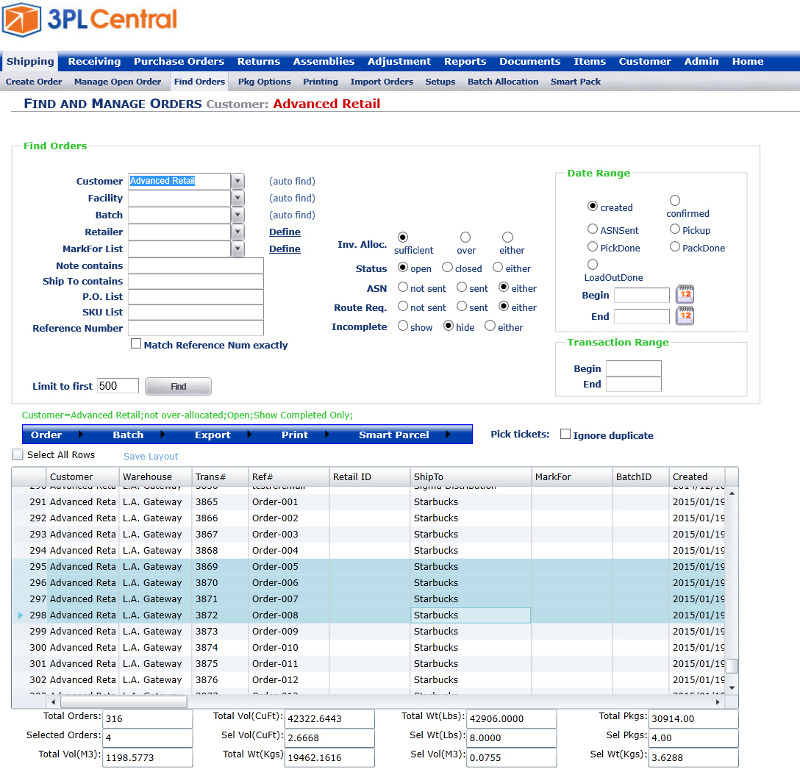
\includegraphics[scale=0.35]{imagenes/estudioArte/pl-800.png}
\caption{ 3PL Cental  }  
\end{figure} 



\subsection{Windward System Five's Inventory Control}


Windward System Five's Inventory Control\cite{wws} diseñado en principio para gestionar inventarios de negocios con E-commerce, utiliza un sistema de códigos de barras para facilitar el pago, cuenta con procesamiento integrado de tarjeta de crédito y utiliza aplicaciones móviles pero no para la gestión, si no para las ventas. Su principal desentaja es el precio, el paquete básico de servicios ronda entorno a los 4300\$

\begin{figure}[htbpH]  
\centering 
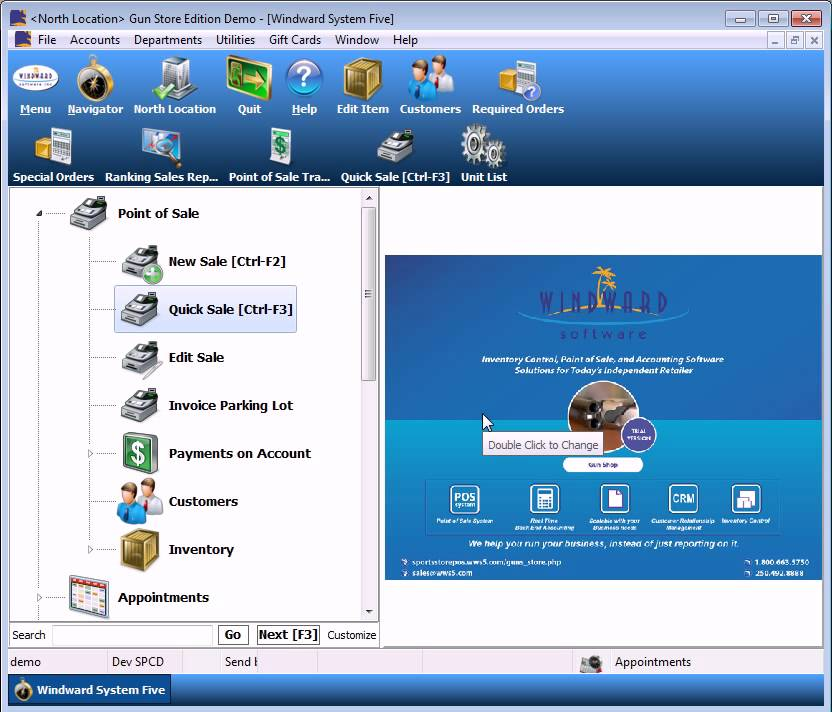
\includegraphics[scale=0.35]{imagenes/estudioArte/five.jpg}
\caption{Windward System Five's}  
\end{figure}

\subsection{Snappii}

Snappii\cite{snp} es una plataforma de desarrollo de aplicaciones a medida para la gestión de almacenes. NO cuenta con plataforma o aplicación de escritorio propiamente dicha. Proporciona aplicaciones ya desarrolladas o la posibilidad de crear nuevas que se ajusten alas necesidades del negocio. Plataforma Android e IOS. El paquete básico de servicios ronda entorno a los 50\$ al mes

\begin{figure}[htbpH]  
\centering 
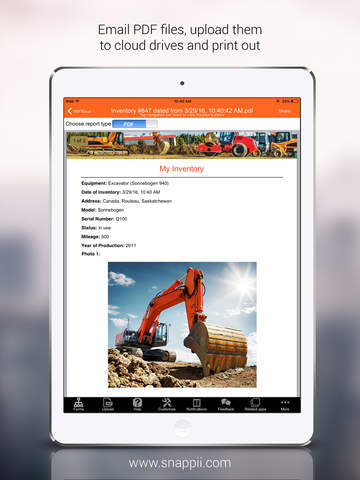
\includegraphics[scale=0.5]{imagenes/estudioArte/shapi.jpeg}
\caption{Snappii}  
\end{figure}




\subsection{Conclusiones}

De todos estos productos, podemos destacar puntos fuertes como estar alojados en la nube, utilizar tecnologías de radiofrecuencia o tecnologías móviles para la gestión. Otros aspectos importantes son la automatización de tareas, controlar el flujo de entrada/salida de objetos o la generación de informes pero también presentan aspectos negativos como son el precio de los servicios o las complicadas interfaces que no facilitan su uso para empleados poco cualificados. 

Estas conclusiones  han sido de gran utilidad para el siguiente capítulo en el que se detallará el proceso de análisis y especificación del sistema final.  

\chapter{Planificación y Costes}

\section{Planificación}

Una vez definidos los objetivos a cumplir para el proyecto, se presenta la planificación temporal a cumplir en forma de diagrama de Gantt. Dicho diagrama ha sido dividido en 4 partes para facilitar su comprensión. Ha sido realizado con la herramienta online Tom's Planner\cite{tomsplanner}

La primera fase del proyecto se basa en recabar información. Realizar un estudio del arte con el objetivo de identificar las ventajas e inconvenientes de algunos sistemas de almacén, analizar el problema, realizar el análisis de requisitos, la creación de los repositorios para el control de versiones y la creación de diversas redes sociales como son el blog\cite{blog} del proyecto y su perfil\cite{twitter} de Twitter. 

\begin{figure}[H] 
\centering 
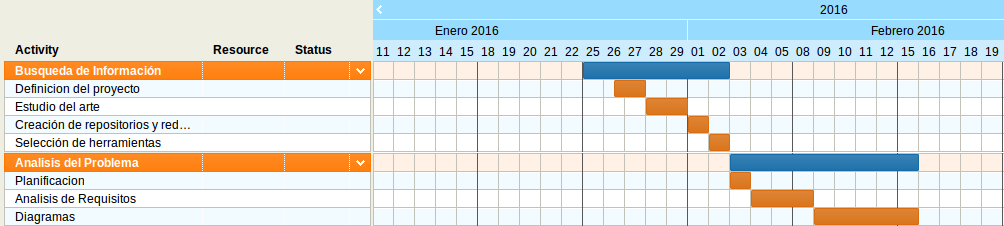
\includegraphics[scale=0.45]{imagenes/planificacion/planificacion1.png}
\caption{ Fase 1 - Planificación\cite{propio}  }  
\end{figure}

La segunda fase del proyecto corresponde con el comienzo del desarrollo de un prototipo de la plataforma web y de la aplicación Android basándose en el análisis y especificación de requisitos. Un prototipo que permita interactuar a los dos subsistemas siempre y cuando estén conectados a la misma red local.

\begin{figure}[H] 
\centering 
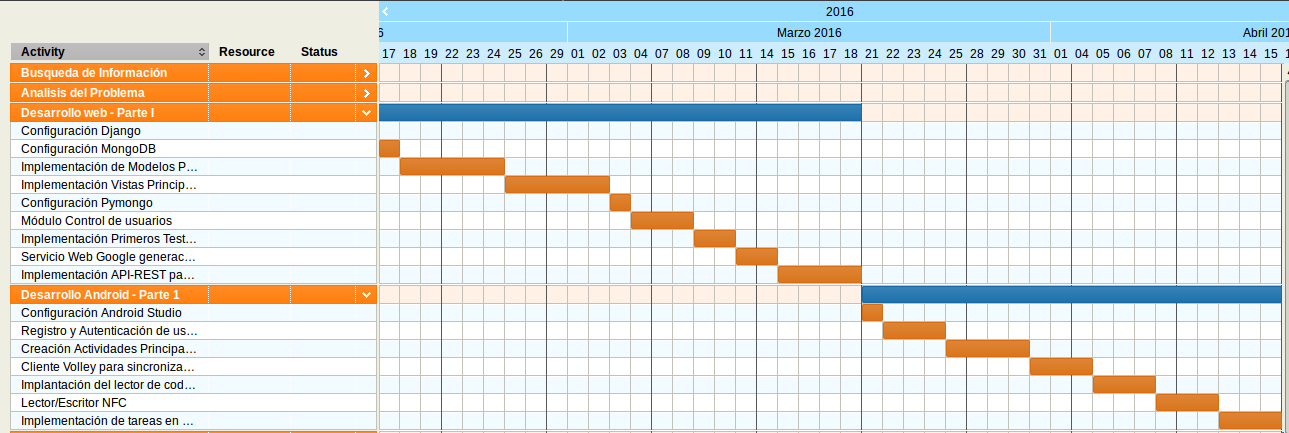
\includegraphics[scale=0.45]{imagenes/planificacion/planificacion2.png}
\caption{ Fase 2 - Planificación\cite{propio}  }  
\end{figure}

La tercera fase de planificación se centra en completar el desarrollo web y principalmente en la creación de toda la infraestructura de la plataforma

\begin{figure}[H] 
\centering 
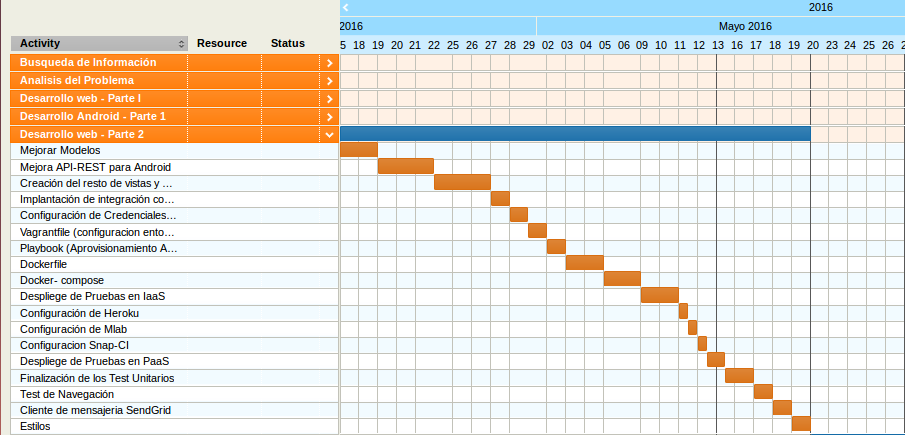
\includegraphics[scale=0.45]{imagenes/planificacion/planificacion3.png}
\caption{ Fase 3 - Planificación\cite{propio}  }  
\end{figure}

La cuarta y última fase de la planificación se basa en la documentación del proyecto, en pulir ciertos aspectos de la aplicación Android y en testear el sistema completo (plataforma web + aplicación Android) desplegado en la nube. 

\begin{figure}[H] 
\centering 
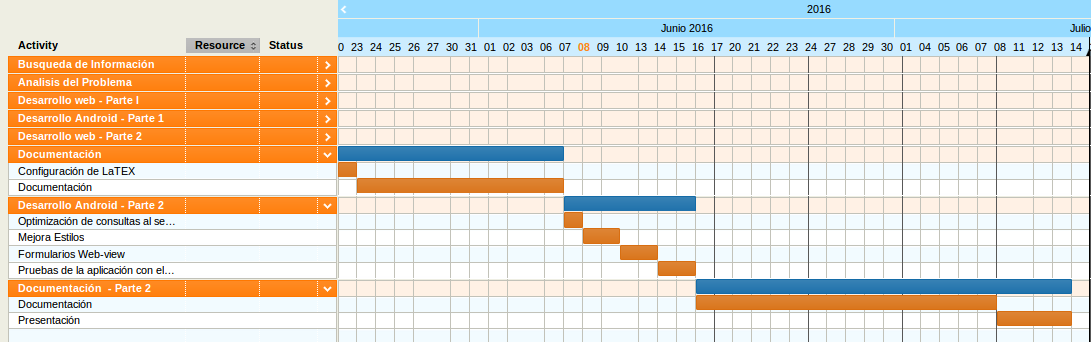
\includegraphics[scale=0.45]{imagenes/planificacion/planificacion4.png}
\caption{ Fase 4 - Planificación\cite{propio}  }  
\end{figure}

\section{Costes}

\chapter{Análisis}

Para realizar un mejor análisis del sistema, vamos a desglosarlo en dos partes. Primero analizaremos la plataforma web y después analizaremos la aplicación Android 

\section{Analisis Plataforma Web}
\subsection{Requisitos de Información Plataforma web}

Los requisitos de información se caracterizan por  reunir la información 	relevante para el cliente que debe gestionar y almacenar el sistema software.\par 

\textbf{RI-1. Item:} Representación de cada uno de los elementos en el sistema. 
Contenido: nombre, descripción, fecha de alta, ID, Localizador, organización de la que forma parte, el usuario que lo dio de alta, atributos. Los atributos son una tupla de 3 valores asignados en función de las preferencias con las que se quiera clasificar  cada elemento. Por ejemplo lugar del que procede, tipo de elemento y estado del elemento.


\textbf{RI-2. Catalogo:} Representación de cada una de las colecciones de elementos del sistema. Contenido: nombre, descripción, fecha de alta, ID, mensaje de aviso, fecha de expiración, tipo de catalogo,  organización de la que forma parte, el usuario que lo dio de alta, colección con las ID de los elementos que forman el catalogo.

\textbf{RI-3. Gráfico:} Información del estado del sistema en forma de grafico, en función de los catálogos creados por los distintos usuarios de una misma organización. Gráficos representativos basados en los atributos de los items que forman cada catalogo. Comparativa entre unidades y peso de esas unidades en el catalogo. 
Contenido: catalogo.

\textbf{RI-4. Informe:} Información del estado del sistema en forma de documento. Generado en función de los catálogos creados por los distintos usuarios de una misma organización y de los gráficos representativos. 
Contenido: nombre, fecha de creación, usuario, organización, datos del informe. 

\textbf{RI-5. Perfil de Usuario:} Información sensible del usuario que va a trabajar con el sistema. Contenido: nombre de usuario, contraseña, correo electrónico, organización. 

\textbf{RI-6. Preferencias:} Información de los atributos que se desean utilizar para clasificar los elementos del sistema dentro del entorno colaborativo de la organización.
Contenido: archivo csv de preferencias 1, archivo csv de preferencias 2, archivo csv de preferencias 3. 


\subsection{Requisitos Funcionales Plataforma web}

Como se define en la ingeniería de requisitos, los requisitos funcionales establecen los comportamientos del sistema.

\textbf{RF-1. Gestión de items:} El sistema deberá gestionar el ciclo de vida de items o elementos existentes en el sistema.
   

	RF-1.1. El sistema permitirá añadir items

	RF-1.2. El sistema permitirá buscar items

	RF-1.3. El sistema permitirá modificar items

	RF-1.4. El sistema permitirá eliminar items

	RF-1.5. El sistema permitirá agrupar items en colecciones


\textbf{RF-2. Gestión de catálogos:} El sistema deberá gestionar el ciclo de vida de conjuntos de items, estas colecciones reciben el nombre de catálogos o agrupaciones de items con atributos u objetivos similares.   


	RF-2.1. El sistema permitirá añadir catálogos

	RF-2.2. El sistema permitirá buscar catálogos

	RF-2.3. El sistema permitirá modificar catálogos

	RF-2.4. El sistema permitirá eliminar catálogos

	RF-2.5. El sistema permitirá limpiar catálogos

	RF-2.6. El sistema permitirá eliminar un item del catalogo

	RF-2.7. El sistema permitirá exportar los códigos qr de sus elementos

	RF-2.8. El sistema permitirá exportar los códigos de barras de sus elementos

	RF-2.9. El sistema permitirá controlar el peso de los elementos del catálogo

	RF-2.10. El sistema permitirá controlar el número de unidades del catálogo. 
	

\textbf{RF-3. Gestión de Gráficos:} El sistema deberá generar gráficos a raíz de los elementos que forman parte de un catálogo, mostrando una comparativa entre el numero de unidades y peso de dichas unidades. Los gráficos representativos se dividen en función de las preferencias del usuario. 


	RF-3.1. El sistema permitirá generar gráficos
	
	RF-3.1. El sistema permitirá exportar gráficos
	
	RF-3.1. El sistema permitirá seleccionar el tipo de gráfico	


	 
\textbf{RF-4. Gestión de Informes:} El sistema deberá generar informes significativos a raíz de los elementos que forman parte de un catálogo. El sistema proveerá al usuario de una plantilla editable para personalizar los aspectos e información necesaria para el informe. El sistema permitirá combinar distintos catálogos para generar un mismo informe.  El sistema permitirá incluir en los informes, los gráficos generados con anterioridad. 

	

	RF-4.1. El sistema permitirá generar informes
	
	RF-4.2. El sistema permitirá almacenar informes
	
	RF-4.3. El sistema permitirá modificar informes
	
	RF-4.4. El sistema permitirá eliminar informes
	
	RF-4.5. El sistema permitirá añadir catálogos a los informes
	
	RF-4.6. El sistema permitirá añadir gráficos a los informes
	
	RF-4.7. El sistema permitirá exportar informes
	

\textbf{RF-5. Gestión de Preferencias:} El sistema permitirá personalizar las preferencias de cada organización. Dichas preferencias son los atributos con los que van a catalogarse los items. Dichos atributos son los que se usarán para dotar de contenido a los catálogos. Estos atributos también son empleados para la generación de gráficos. 


	RF-5.1. El sistema permitirá cargar las preferencias desde fichero CSV
	
	RF-5.1. El sistema permitirá cargar preferencias por defecto 
	
	

\textbf{RF-6. Gestión de Usuarios:} El sistema deberá presentar un entorno colaborativo, clasificando a los usuarios por organizaciones de forma que distintos usuarios de una misma organización tengan acceso al mismo conjunto de recursos que define dicha organización. 


	RF-6.1. El sistema permitirá al administrador dar de alta a nuevos usuarios.
	
	RF-6.1. El sistema permitirá al administrador asignar perfiles de usuario.
	
	RF-6.2. El sistema permitirá iniciar sesión a los usuario.
	
	RF-6.2. El sistema permitirá cerrar sesión a los usuario.
	
	RF-6.2. El sistema registrará internamente las acciones realizadas por cada 	usuario, 	de cada organización. 
	
	

\subsection{Requisitos No Funcionales Plataforma web}
Los requisitos no funcionales, se refieren a todos los requisitos que no describen información a guardar, ni funciones a realizar por el sistema, sino características de funcionamiento.


\textbf{RNF-1} Necesitaremos que toda la información que se almacena sobre el sistema se mantenga segura, realizando copias de seguridad periódicas.


\textbf{RNF-2} Necesitaremos analizar la cantidad de elementos que una organización va a administrar. Si es considerada una cantidad importante, dicha organización recibirá servicio desde una imagen del sistema asilada (Docker). De esta forma conseguimos que el flujo de datos no afectes a la experiencia de los clientes.


\textbf{RNF-3} Necesitaremos disponer de una buena conexión a internet ya que el sistema da servicio desde la nube. 



\subsection{Casos de Uso: Plataforma Web}

Los diagramas de casos de uso, son diagramas UML que representan gráficamente a todos los elementos que forman parte del modelo de casos de uso junto con la frontera del sistema. Delimitan el sistema a diseñar. Determinan el contexto del uso del sistema. Describen el punto de vista de los usuarios  en el sistema 

\begin{figure}[htbpH]  
\centering 
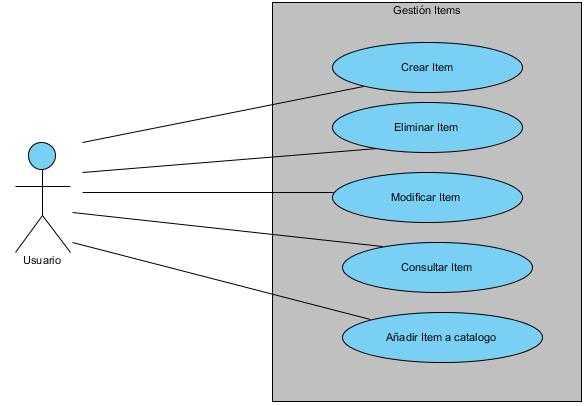
\includegraphics[scale=0.50]{imagenes/casosUso/gestionItem.jpg}
\caption{ Casos de uso - Gestión Items  }  
\end{figure}

\begin{figure}[H] 
\centering 
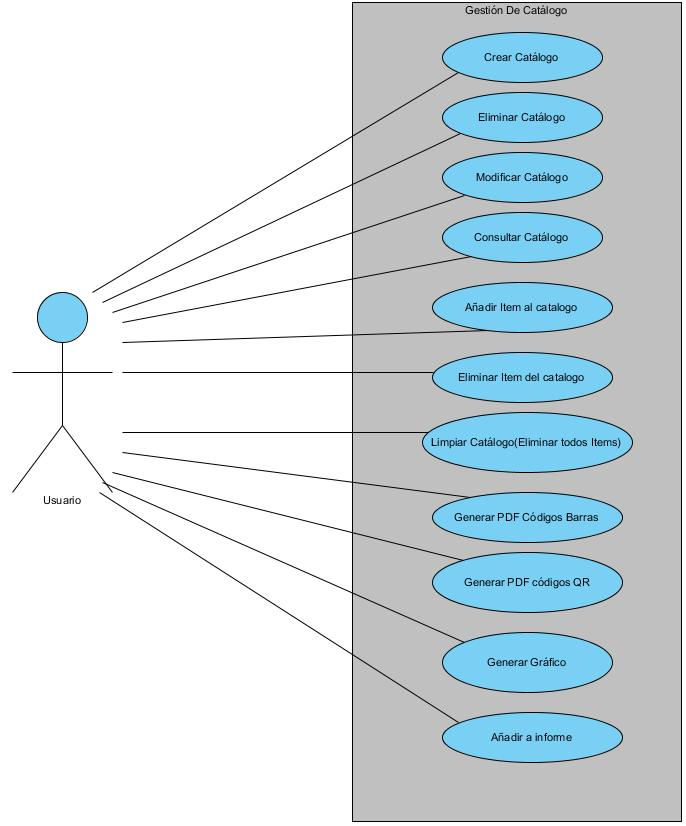
\includegraphics[scale=0.50]{imagenes/casosUso/gestionCatalogo.jpg}
\caption{ Casos de uso - Gestión Catalogos  }  
\end{figure}


\begin{figure}[H] 
\centering 
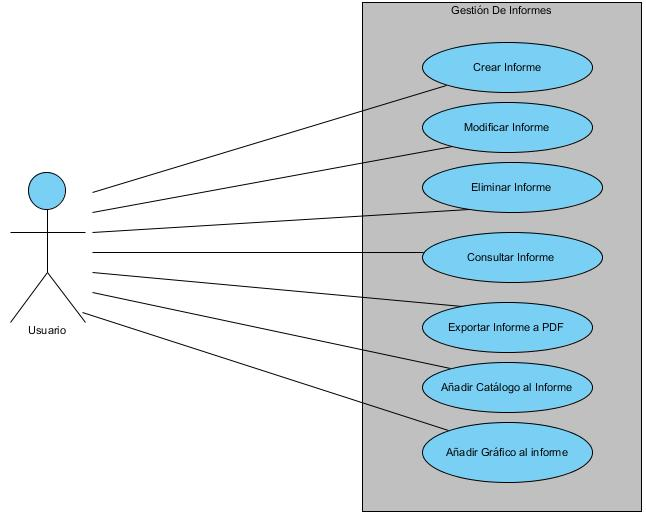
\includegraphics[scale=0.50]{imagenes/casosUso/Informe.jpg}
\caption{ Casos de uso - Gestión Informes  }  
\end{figure}

\section{Analisis Aplicación Android}
\subsection{Requisitos Funcionales Aplicación Android}
Los requisitos funcionales de la aplicación Android establecen los comportamientos o funcionalidades de la aplicación.

\textbf{RF-1. Administración de items} La aplicación deberá administrar los items que formen parte del almacen.   


	RF-1.1. La aplicación permitirá detectar items mediante texto o localizador
	
	RF-1.2. La aplicación permitirá detectar items mediante codigo QR
	
	RF-1.3. La aplicación permitirá detectar items mediante codigo de barras
	
	RF-1.4. La aplicación permitirá detectar items mediante etiquetas NFC
	
	RF-1.5. La aplicación permitirá escribir el localizador de un item en una etiqueta NFC
	
	RF-1.6. La aplicación permitirá consultar un item en detalle
	
	RF-1.7. La aplicación permitirá añadir un item detectado a un catalogo determinado
	
	RF-1.8. La aplicación permitirá eliminar items


\textbf{RF-2. Administración de Catálogos}La aplicación deberá administrar los catálogos que se utilicen para clasificar los items del almacén.   


	RF-2.1. La aplicación permitirá detectar catálogos mediante texto o ID
	
	RF-2.2. La aplicación permitirá añadir items  al catalogo mediante código QR
	
	RF-2.3. La aplicación permitirá añadir items al catalogo mediante código de barra
	s
	RF-2.4. La aplicación permitirá añadir items al catalogo mediante etiquetas NFC
	
	RF-2.5. La aplicación permitirá eliminar items de un catalogo
	
	RF-2.6. La aplicación permitirá limpiar la lista de items de un catalogo
	
	
\textbf{RF-3. Sesión de Usuario} La aplicación deberá identificar a cada usuario de manera única para certificar las tareas de administración que se lleven acabo desde la aplicación. 


	RF-3.1. La aplicación permitirá al usuario iniciar sesión.
	
	RF-3.2. La aplicación permitirá al usuario cerrar sesión.



\chapter{Desarrollo del sistema}



\section{Dessarrollo web}
En esta parte se abordarán los aspectos mas importantes de la plataforma web. Que tecnologías has sido utilizadas, como han sido utilizadas y por qué han sido utilizadas.

\subsection{Django}
Django\cite{dj}, es un Framework de alto nivel para Python. Django sigue la metodología de diseño “Modelo Vista Controlador” (MVC) lo que permite crear aplicaciones web extensibles, escalables y sostenibles. Django es de código abierto. 

Django cuenta con varios módulos para asegurar la seguridad e integridad de las aplicaciones web desarrolladas con el. 

Django posee un sistema jerárquico de plantillas que facilita la reutilización de código y extensibilidad de aplicaciones. Además cuenta con soporte para internacionalización.

En este proyecto se ha decidido utilizar Django debido a que utiliza python y que además al ser un framework de alto nivel, reúne diversas herramientas y aplicaciones, como por ejemplo el servidor de aplicación para desarrollo que facilita el trabajo para desarrollar de manera ágil, el modulo de autenticación de usuarios, el modulo para desarrollo baso en test o la integración de servicios de mensajería de manera interna. Al principio se planteaba realizar la plataforma web con PHP pero al ser un sistema bastante grande, se decidió optar por Django ya que facilitaba el proceso de desarrollo. También se pensó en el micro-framework python Flask pero después del proceso de análisis, se llegó a la conclusión de que con Flask\cite{fl} se repetiría mucho mas código y con Django el diseño seria también más escalable.

\subsection{MongoDB}

MongoDB\cite{mg} es un sistema de base de datos NoSQL orientado a grandes cantidades de datos, guarda estructuras de datos en documentos similares a JSON haciendo que la integración de los datos en ciertas aplicaciones sea más fácil y rápida.
Se trata de una base de datos ágil que permite cambiar los esquemas de una aplicación cuando esta evoluciona. Los principales objetivos de estas bases de datos son la escalabilidad, rendimiento y gran disponibilidad.

En MongoDB los documentos se agrupan en colecciones. Las colecciones  no imponen una estructura fija a los documentos que contienen, ni siquiera al tipo de datos de cada campo. Esto es una ventaja cuando estamos desarrollado un sistema en el que las entradas de la base de datos dependen de las preferencias del usuario.

\begin{figure}[H] 
\centering 

\includegraphics[scale=0.45]{imagenes/desarrollo_herramienta/mongo.png}
\caption{ MongoDB-Logo\cite{mongoL}  }  
\end{figure} 

Las principales características de las bases de datos no relacionales como MongoDB son la velocidad y la flexibilidad. La eficiencia en las consultas sobre bases de datos no relacionales, y mas aun, cuando estas consultas marcan la calidad de experiencia que percibe el usuario, ya sea en el portal web o en la aplicación Android.  Las tareas de consulta, inserción, modificación o borrado presentan una gran eficiencia ya que pueden ser realizadas mediante funciones JavaScript en el cliente, conectando directamente con la base de datos.

En cuanto a la flexibilidad, la principal ventaja es la escalabilidad, por ejemplo, en el momento en que un usuario necesite mas atributos para clasificar sus objetos, lo que en el mundo de las bases de datos relacionales se traduciría en agregar mas columnas a las tablas que representan todos los objetos, cuando se trabaja con bases de datos no relacionales esto no es un impedimento, ya que en la misma colección pueden convivir documentos u objetos con distintos campos o valores. Esto es perfecto para darle al usuario la libertad de personalizar los atributos con los que quiere identificar sus objetos. 

Las consultas sobre MongoDB son consultas Ad Hoc, las cuales soportan búsqueda por campos, consultas por rangos y expresiones regulares. También pueden ser funciones JavasScript definidas por el desarrollador. 

Cualquier documento de MongoDB puede ser indexado. Los índices funcionan de manera similar a los de las bases de datos relacionales. 

En cuanto a la replicación y Balanceo de carga, MongoDb soporta el paradigma maestro-esclavo. Es capaz de escalar horizontalmente y tiene la capacidad de ejecutarse en múltiples servidores, balanceando la carga y duplicando de datos para garantizar el funcionamiento del sistema en caso de fallo. 

En MongoDB, los documentos los guarda en BSON, que es una forma de representar de forma binaria objetos JSON. Un ejemplo de documento almacenado en MongoDB que representa a un item del almacén, es el siguiente:

\begin{figure}[H] 
\centering 
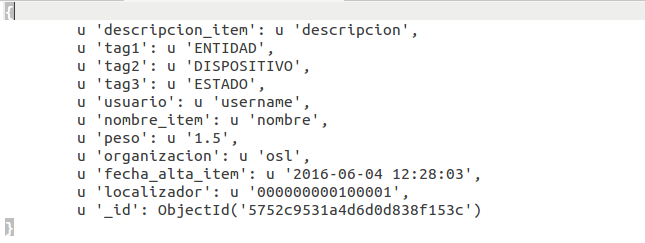
\includegraphics[scale=0.45]{imagenes/desarrollo_herramienta/bson.png}
\caption{ Ejemplo Bson\cite{propio}}  
\end{figure} 

Este documento es básico. Los documentos pueden anidarse, dando lugar a documentos mas complejos con muchas mas información. Pueden contener también listas de otros elementos o valores. 

\subsection{Pymongo} 
Pymongo\cite{pymongo} es un paquete python que facilita un cliente o driver intermediario para controlar la iteración del sistema con la base de datos MongoDB. Algunas de las características que Pymongo ofrece son:

\begin{enumerate}
\item Conexión con la Base de Datos
\item Visualización de las Bases de Datos creadas.
\item Creación de nuevas Bases de Datos
\item Visualización de las colecciones creadas
\item Creación de nuevas colecciones
\item Inserción de nuevos documentos
\item Actualización de documentos
\item Búsqueda de documentos
\item Eliminación de documentos
\end{enumerate}

Pymongo es el controlador que permite a nuestro modelos interaccionar con la base de datos, de esta manera se consigue utilizar Django, que esta pensado para bases de datos relacionales, con MongoDB que es una base de datos no relacional ya que funciona como intermediario entre los modelos de objetos creados de manera externa al framework y la base de datos.

\begin{figure}[H] 
\centering 

\includegraphics[scale=0.25]{imagenes/desarrollo_herramienta/pymongo.jpg}
\caption{ Logo Pymongo\cite{pymongoL}}  
\end{figure} 

 

\subsection{JQuery}

JQuery\cite{jq} es una librería de JavaScript, que permite interactuar con los documentos HTML, manipular el árbol DOM, manejar eventos, desarrollar animaciones y agregar interacción con el servidor mediante llamadas asíncronas realizadas con Ajax. Su objetivo principal es dar un comportamiento dinámico a las paginas web. Jquery funciona en múltiples navegadores, ya que es compatible con CSS3.

\begin{figure}[H] 
\centering 

\includegraphics[scale=0.25]{imagenes/desarrollo_herramienta/JQuery.png}
\caption{ JQuery-Logo\cite{jq2}  }  
\end{figure}   

En este proyecto, el principal uso de Jquery se realiza junto con Ajax para recargar la información de la web de manera dinámica mediante llamadas asíncronas. El uso de estas tecnologías mejora la experiencia del usuario cuando interactúa con el sistema mediante la plataforma web y la aplicación Android.


\subsection{Bootstrap}
Bootstrap\cite{boo} es un framework CSS para dar forma a sitios web mediante librerías CSS. Bootstrap  permite crear interfaces de usuario limpias y totalmente adaptables a todo tipo de dispositivos y pantallas ya que esta caracterizado por ser responsive. Es compatible con los siguientes navegadores: 

\begin{enumerate}
\item Google Chrome
\item Safari
\item Mozilla Firefox 
\item Internet Explorer 
\item Opera  
\end{enumerate}

\begin{figure}[H] 
\centering 

\includegraphics[scale=0.25]{imagenes/desarrollo_herramienta/bootstrap.png}
\caption{ Bootstrap-Logo\cite{booL}  }  
\end{figure}   
 
 
\section{Infraestructura}
\subsection{Plataforma Como Servicio}

La Plataforma como Servicio\cite{paas} (PaaS, Platform as a Service) es una categoría de servicios cloud que proporciona un entorno a los desarrolladores crear aplicaciones y servicios que funcionen a través de internet. Los servicios PaaS se alojan en la nube, y los usuarios pueden acceder a ellos a través de un navegador web. . Los servicios PaaS consisten en funcionalidades preconfiguradas a las que los clientes puedan suscribirse, eligiendo las funciones que deseen incluir en función de sus necesidades.

Algunas de las funcionalidades PaaS son:

\begin{enumerate}
\item Sistema operativo 
\item Entorno de scripting de servidor 
\item Sistema de gestión de base de datos 
\item Software de servidor 
\item Soporte técnico 
\item Almacenamiento 
\item Acceso a la red 
\item Herramientas de diseño y desarrollo 
\item Hosting 
\end{enumerate}

Para Realizar el despliegue de este proyecto en un PaaS se ha utilizado Heroku\cite{hero}. Heroku es una plataforma en la nube basado en un sistema de contenedores gestionados, con servicios de datos integrados y un potente ecosistema, para implementar y ejecutar aplicaciones modernas. Heroku presenta una fácil integración con github y por es de carácter gratuito (al menos algunos servicios). Heroku se caracteriza por el fichero de configuración denominado Procfile. Dicho fichero, se encarga de arrancar una instancia web y dejar que gunicorn (servidor de aplicación) ejecute el sistema en ella.

Otro motivo por el cual usar Heroku es por la automatización del despliegue. Heroku nos facilita un repositorio para almacenar el sistema. Un complemento para realizar despliegues en Heroku de forma automatizada es el sistema de integración continua Snap-CI\cite{snap}.  Como podemos observar en la siguiente captura, Snap-CI nos permite vincular el repositorio en el que se encuentra el sistema y desglosar en un pipeline los distintos estados por los que pasa el despliegue, pasando por la instalación de dependencias y ejecución de los test para integración continua hasta despliegue con Heroku.  

\begin{figure}[h] 
\centering 
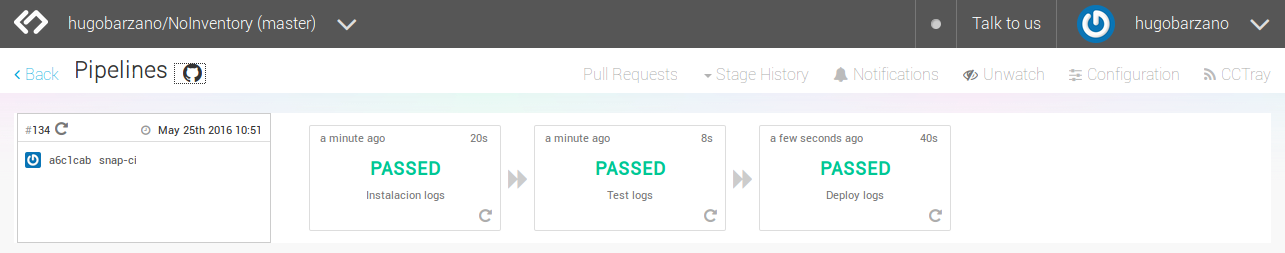
\includegraphics[scale=0.25]{imagenes/desarrollo_herramienta/snp_ci.png}
\caption{ Pipeline Snap-CI  }  
\end{figure}

\subsection{Infraestructura Como Servicio}
La Infraestructura como Servicio\cite{iaas} (IaaS, Infrastructure as a Service) es un servicio cloud, que proporciona acceso a recursos informáticos situados en un entorno virtualizado, a través de una conexión pública. Los recursos informáticos ofrecidos  son básicamente infraestructura de procesamiento. Físicamente, el repertorio de recursos hardware disponibles procede de multitud de servidores y redes, generalmente distribuidos entre numerosos centros de datos, de cuyo mantenimiento se encarga el proveedor del servicio cloud. El cliente, por su parte, obtiene acceso a los componentes virtualizados para construir con ellos su propia plataforma informática.

Estas son las ventajas características de una implementación basada en el modelo de Infraestructura como Servicio:

\begin{enumerate}
\item Escalabilidad
\item Sin necesidad de invertir en hardware
\item Independencia de la localización
\item Seguridad física en los centros de datos
\end{enumerate}

\subsection{Docker}

Docker\cite{dk} es una herramienta para automatizar el despliegue de aplicaciones dentro de contenedores, proporcionando una capa de abstracción y automatización de Virtualización a nivel de sistema operativo. Docker utiliza aislamiento de recursos del kernel de Linux, para permitir que contenedores independientes se ejecuten dentro de una sola instancia de Linux, evitando la sobrecarga de iniciar y mantener máquinas virtuales.

\begin{figure}[h] 
\centering 
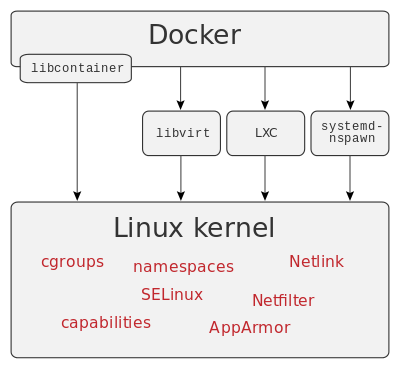
\includegraphics[scale=0.35]{imagenes/desarrollo_herramienta/docker.png}
\caption{ Virtualización Docker\cite{dkw}}
\end{figure}

La principal diferencia con respecto a maquinas virtuales es el tamaño. Las maquinas virtuales incluyen la aplicación, el codigos, las libresrias necesarias y un sistema operativo anfitrion completo mientras que los contenedores contienen los mismo pero comparten el nucleo con otros contenedores corriendo como una proceso asilado en el espacio de usuario del sistema operativo anfitrion. No estan vinculados con ninguna infraestructura especifica 

\subsection{Ansible}

Ansible\cite{ans} es una herramienta de automatización que permite configurar sistemas, implementar software y orquestar tareas complejas como por ejemplo despliegues continuos. En este proyecto se ha decidido utilizar Ansible como mecanismo de aprovisionamiento de aplicación, debido a su fiabilidad, facilidad de uso y seguridad. Para poder trabajar con Ansible es necesario crear playbooks que no son mas que archivos de aprovisionamiento.yml en los que detallar todas las dependencias, servicios y tareas que nuestra aplicación necesita para funcionar. Aunque puede usarse de manera independiente, si la combinamos con herramientas de creación y administración de entornos virtuales como por ejemplo Vagrant, podemos llegar a conseguir grandes resultados.

\begin{figure}[H] 
\centering 
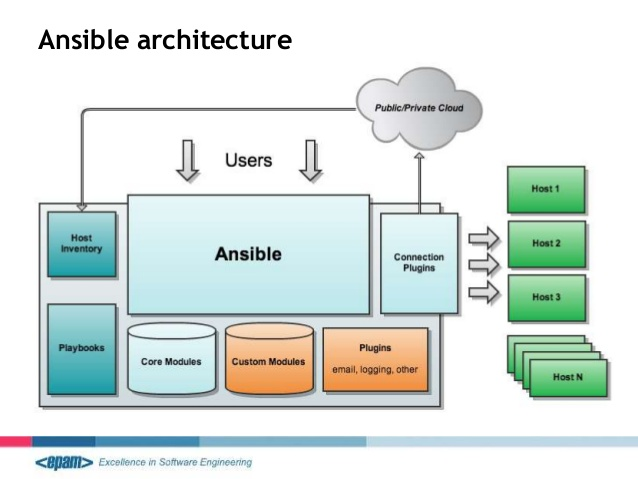
\includegraphics[scale=0.35]{imagenes/desarrollo_herramienta/ansible.jpg}
\caption{ Arquitectura Ansible\cite{ans2}}
\end{figure}

\subsection{Vagrant}

Vagrant\cite{vg} es una herramienta open-source para la creación y configuración de entornos de desarrollo virtualizados. Vagrant proporciona entornos de trabajo fáciles de configurar, reproducibles y portátiles. Está desarrollado con Ruby y utiliza el sistema de virtualización Virtualbox de Oracle. Este proyecto tiene asociado un fichero denominado Vagrantfile cuya función principal es la de describir el tipo de máquinas necesarias para la aplicación, cómo configurarlas y como aprovisionarlas. Las posibilidades con Vagrant son muy numerosas, en este proyecto se va a utilizar Vagrant para la configuración de maquinas virtuales alojadas en Azure. Dichas maquinas correrán directamente con la aplicación utilizando Ansible y también correrán con la aplicación de manera asilada utilizando contenedores. 

\begin{figure}[H] 
\centering 
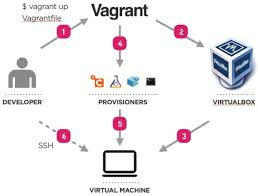
\includegraphics[scale=0.75]{imagenes/desarrollo_herramienta/vagrant.jpeg}
\caption{ Funcionamiento Vagrant\cite{vg2}}
\end{figure}


Dependiendo del proveedor de servicio, Vagrant será configurado de una manera u otra. En este proyecto se va a utilizar Azure, por lo que Vagrant necesita el plugin Microsoft Azure provider to Vagrant. Con este plugin detallamos entre otras cosas las credenciales necesarias para autenticación en Azure.

Vagrant cuenta con infinidad de plugins para distintos cloud services y distintos entornos de de desarrollo virtuales. Con Vagrant no solo podemos trabajar individualmente maquina a máquina, podemos utilizar la caracteristica vagrant-multimachine para crear en paralelo N máquinas virtuales y aprovisionarlas cada una como queramos. 


\section{Desarrollo Android}

Android es un sistema operativo basado en el núcleo Linux diseñado inicialmente para teléfonos móviles, al igual que iOS, Symbian y Blackberry OS. El sistema permite programar aplicaciones en una variación de Java llamada Dalvik. El sistema operativo proporciona todas las interfaces necesarias para desarrollar aplicaciones que accedan a las funciones del teléfono. 

En esta sección se hablará del entorno de programación utilizado para desarrollar la aplicación Android, así como de las tecnologías utilizadas en la aplicación para mantener la sincronización con la plataforma web y llevar a cabo las tareas de clasificación.  

\subsection{Android-Studio}

Para trabajar con Android hay diversos entornos de desarrollo como por ejemplo Eclipse, pero el mas recomendado y el utilizado en este proyecto es Android Studio\cite{as}. Android Studio es un entorno de desarrollo integrado (IDE), basado en IntelliJ IDEA de la compañía JetBrains,  que proporciona varias mejoras con respecto al plugin ADT (Android Developer Tools) para Eclipse. Android Studio utiliza una licencia de software libre Apache 2.0

\begin{figure}[H] 
\centering 

\includegraphics[scale=0.5]{imagenes/desarrollo_herramienta/android.png}
\caption{ Android-Studio}
\end{figure}


Algunas características\cite{as2} de este entorno de programación son:

\begin{enumerate}
\item Soporte para programar aplicaciones para Android Wear.
\item Herramientas Lint para detectar problemas de rendimiento, usabilidad y compatibilidad de versiones.
\item Utiliza ProGuard para optimizar y reducir el código del proyecto al exportar a APK.\item Integración de la herramienta Gradle encargada de gestionar y automatizar la construcción de proyectos.
\item Nuevo diseño del editor con soporte para la edición de temas. 
\item Nueva interfaz específica para el desarrollo en Android.
\item control de versiones accediendo a un repositorio desde el que poder descargar Mercurial, Git, Github o Subversion. 
\end{enumerate}

\subsection{Librería Volley}
La aplicación No-inventory-Android-App, sirve como extensión de la plataforma web. Esta aplicación esta sincronizada en tiempo real con el servidor de manera que la experiencia de usuario entre la web y la aplicación es óptima.  Para conseguir esto, se utiliza la librería Volley\cite{volley} desarrollada por Google con el objetivo de optimizar el envío de peticiones Http desde las aplicaciones Android hacia servidores externos. Actúa como una interfaz de alto nivel, liberando al programador de la administración de hilos y procesos de parsing. 


\begin{figure}[H] 
\centering 
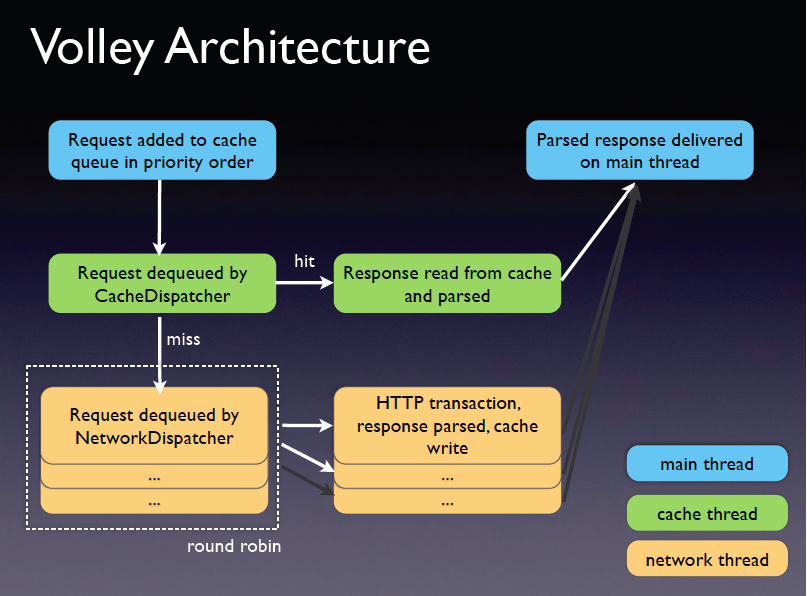
\includegraphics[scale=0.5]{imagenes/desarrollo_herramienta/volley.png}
\caption{ Arquitectura Volley\cite{volley2}}
\end{figure}

Volley funciona mediante una arquitectura a capas, en la que cada capa está representada por una hebra. Se puede distinguir entre la hebra principal de la aplicación, la hebra de cache y la hebra que se encarga de realizar las peticiones HTTP.  Las peticiones son añadidas a una cola con prioridad y van siendo atendidas en función de los requisitos de la hebra principal. En el caso de que los datos no estén cacheados, la hebra de cache envía la petición a la hebra de transacción y esta realiza la petición. Un problema importante a la hora utilizar Volley en esta aplicación fue la congestión de la red, ya que cada petición Volley creaba una cola de peticiones propia para cada consulta. La solución tomada fue la de implementar esta cola como estática de manera que todas las peticiones que se llevan a cabo en las distintas vistas de la aplicación, comparten la cola de peticiones, mejorando así el rendimiento y evitando problemas de sobre carga de memoria ya que Volley lo cachea todo. 


\subsection{Near field communication (NFC)}
NFC\cite{nfc} o comunicación de campo cercano, es una tecnología inalámbrica derivada de la etiquetas RFID. NFC es una plataforma abierta pensada para teléfonos  y dispositivos móviles. Su tasa de trasferencia ronda entono a los  424 kbit/s por lo que es ideal para la comunicación instanatea aunque como su propio nombre indica, su radio de acción esta entorno a los 10 o 15 cm aunque no necesita emparejamiento previo. 

La tecnología NFC puede funcionar en dos modos:

\begin{enumerate}
\item Activo, en el que ambos equipos con NFC intercambian datos. 
\item Pasivo, en el que solo hay un dispositivo activo y el otro aprovecha el campo magnético generado por este para intercambiar la información.
\end{enumerate}

En este sistema, la aplicación No-inventory-Android-App es capaz de Leer/Escribir etiquetas NFC. Dichas etiquetas contienen el localizador de cada objeto del sistema. De esta manera las tareas de identificación, catalogación y agrupación  se pueden llevar acabo de una manera rápida y eficiente.

\begin{figure}[H] 
\centering 
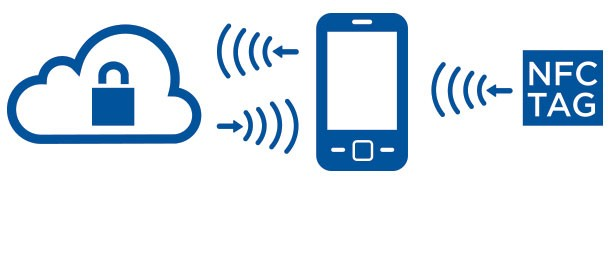
\includegraphics[scale=0.5]{imagenes/desarrollo_herramienta/nfc.jpg}
\caption{ Ejemplo Funcionamiento Etiquetas NFC\cite{nfc4}}
\end{figure}

Para llevar a cabo estas tareas, se ha creado la clase NFC Manager siguiendo los ejemplos de la documentación oficial de Android Developers\cite{nfc2}, con la que controlar las acciones de lectura/escritura y el tipo de etiquetas a escribir. También se usa el Foreground Dispatch System\cite{nfc3} que se encarga de realizar estas tareas en segundo plano  y de establecer la prioridad entre Intens de manera que la lectura/escritura de etiquetas NFC no influya en el hilo de ejecución principal. 


 

\subsection{Lector de Códigos de Barras ZXing}

Otro método de identificación que utiliza  No-inventory-Android-App es la lectura de códigos de barras o códigos QR que contienen, al igual que las etiquetas NFC, el localizador propio de cada objeto dado de alta en el sistema. Son códigos de respuesta rápida, con un coste reducido y con la única necesidad de disponer de una cámara en el Smartphone. 

Para conseguir esto, la aplicación utiliza la librería procesadora de imágenes multi-formato Zxing\cite{cebra}. Esta librería de código abierto  es capaz de reconocer una gran variedad de formatos, como por ejemplo  UPC-A, UPC-E, EAN-8, EAN-13, Códigos 39, 93, 128, ITF, Codabar, RSS-14, Matriz de datos, Aztec, PDF 417 y códigos QR. 

\begin{figure}[H] 
\centering 
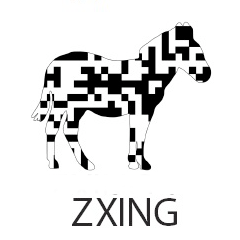
\includegraphics[scale=0.5]{imagenes/desarrollo_herramienta/zxing.png}
\caption{ zxing - logo\cite{cebra3}}
\end{figure}

ZXing ofrece el lector de códigos de barras como una aplicación independiente que, mediante mecanismo de control de Intens\cite{cebra2} permite que otras aplicaciones, como por ejemplo esta,  puedan integrar el lector de manera sencilla.




\chapter{Implementación y pruebas}

\section{Herramientas}
\subsection{Herramientas de infraestructura}


\section{Recursos}

Decir los recursos humanos (autor y directores), hardware y software que se van a utilizar.









\begin{thebibliography}{aaaa}

%estudio del arte
\bibitem[7]{3pl} \textsc{3PL},
\textit{3PL Central}
\url{http://3plcentral.com/} 

\bibitem[8]{wws} \textsc{wws},
\textit{Windward System Five's Inventory Control}
\url{http://www.windwardsoftware.com/en-US/}

\bibitem[8]{snp} \textsc{snp},
\textit{Snappii}
\url{https://www.snappii.com/}

%planificacion
\bibitem[8]{tomsplanner} \textsc{tomsplanner},
\textit{Tom's Planner: Software de planificación}
\url{http://www.tomsplanner.es/}

\bibitem[8]{blog} \textsc{Blog},
\textit{No-Inventory: Blog}
\url{http://no-inventory.es/}

\bibitem[8]{twitter} \textsc{twitter},
\textit{No-Inventory: twitter}
\url{https://twitter.com/no_inventory}

%desarolloweb
\bibitem[8]{dj} \textsc{Django},
\textit{Django}
\url{https://www.djangoproject.com/}

\bibitem[9]{fl} \textsc{Flask},
\textit{Flask}
\url{http://flask.pocoo.org/}

\bibitem[9]{mg} \textsc{mongo},
\textit{MongoDB}
\url{https://www.mongodb.com/}

\bibitem[9]{mongoL} \textsc{mongo-logo},
\textit{MongoDB-Logo}
\url{http://cftic.centrosdeformacion.empleo.madrid.org/web/educamadrid/principal/files/abf76d62-7094-44c2-8970-5ed8387f1cbf/mongodb-logo1.png}

\bibitem[9]{propio} \textsc{propio},
\textit{Elaboración Propia}
\url{}

\bibitem[9]{pymongo} \textsc{pymongo},
\textit{Pymongo Package Index }
\url{https://pypi.python.org/pypi/pymongo/}

\bibitem[9]{pymongoL} \textsc{pymongo-logo},
\textit{pymongo-Logo}
\url{http://easylearning.guru/images/courses/self-paced/pymongo/pymongo.jpg}

\bibitem[9]{jq} \textsc{JQuery},
\textit{JQuery Oficial}
\url{https://jquery.com/}

\bibitem[9]{jq2} \textsc{JQuery Logo},
\textit{JQuery Logo}
\url{https://www.returngis.net/wp-content/uploads/2011/01/JQuery.png}

\bibitem[9]{boo} \textsc{Bootstrap},
\textit{getbootstrap}
\url{http://getbootstrap.com/}

\bibitem[9]{booL} \textsc{Bootstrap Logo},
\textit{Logo}
\url{http://davidgaitan.com/wp-content/uploads/2015/09/singlepro-twitter-bootstrap.png}

%infraestructura

\bibitem[1]{paas} \textsc{PaaS},
\textit{Plataforma como Servicio}
\url{http://www.interoute.es/what-paas} 

\bibitem[2]{hero} \textsc{Heroku},
\textit{Heroku: Plataforma como Servicio}
\url{https://www.heroku.com/}

\bibitem[3]{snap} \textsc{Snap-CI},
\textit{Snap-CI: Sistema Integración Continua}
\url{https://snap-ci.com/}

\bibitem[4]{iaas} \textsc{IaaS},
\textit{Infraestructura como Servicio}
\url{http://www.interoute.es/what-iaas} 


\bibitem[4]{dk} \textsc{Docker},
\textit{Docker - Aislamiento de recursos}
\url{https://www.docker.com/what-docker} 

\bibitem[4]{dkw} \textsc{Docker-Wiki},
\textit{Docker - Wikipedia}
\url{https://es.wikipedia.org/wiki/Docker_\%28software\%29} 


\bibitem[4]{ans} \textsc{Ansible},
\textit{Ansible}
\url{https://www.ansible.com/} 

\bibitem[4]{ans2} \textsc{Ansible},
\textit{Deploying Symfony2 app with Ansible}
\url{http://www.slideshare.net/rodomansky/deploying-symfony2-app-with-ansible} 

\bibitem[4]{vg} \textsc{Vagrant},
\textit{Vagrant}
\url{https://www.vagrantup.com/} 

\bibitem[4]{vg2} \textsc{Vagrant},
\textit{Cómo manejar máquinas virtuales de forma sencilla}
\url{http://www.pixelovers.com/utiliza-vagrant-y-haz-portable-tu-entorno-de-desarrollo/} 


%desarollo android
\bibitem[4]{as} \textsc{Android-Studio},
\textit{Android-Studio-Developer}
\url{https://developer.android.com/studio/index.html?hl=es} 

\bibitem[4]{as2} \textsc{Android-Studio},
\textit{Android-Studio VS Eclipse}
\url{http://academiaandroid.com/android-studio-v1-caracteristicas-comparativa-eclipse/} 

\bibitem[4]{volley} \textsc{Librería Volley},
\textit{Transmitting Network Data Using Volley}
\url{https://developer.android.com/training/volley/index.html?hl=es}

\bibitem[4]{volley2} \textsc{Arquitectura Volley},
\textit{Arquitectura Volley}
\url{https://packetzoom.com/blog/which-android-http-library-to-use.html}

\bibitem[4]{nfc} \textsc{NFC},
\textit{NFC}
\url{http://www.nearfieldcommunication.org/}

\bibitem[4]{nfc2} \textsc{NFC Basico},
\textit{NFC-Basic-Developer}
\url{https://developer.android.com/guide/topics/connectivity/nfc/nfc.html?hl=es}

\bibitem[4]{nfc3} \textsc{ NFC-Foreground Dispatch System },
\textit{NFC -  Foreground Dispatch System}
\url{https://developer.android.com/guide/topics/connectivity/nfc/advanced-nfc.html?hl=es#foreground-dispatch}


\bibitem[4]{nfc4} \textsc{ NFC- Diagrama Ejemplo },
\textit{NFC -  Diagrama Ejemplo}
\url{http://www.secureidnews.com/wp-content/uploads/2014/10/nfc-tag-slider-610x259.jpg}

\bibitem[4]{cebra} \textsc{ Zxing - Proyect},
\textit{Zxing -Zxing}
\url{https://github.com/zxing/zxing}

\bibitem[4]{cebra2} \textsc{ Zxing-Control-Intens},
\textit{Zxing - Stack Overflow}
\url{http://stackoverflow.com/questions/2050263/using-zxing-to-create-an-android-barcode-scanning-app}


\bibitem[4]{cebra3} \textsc{ Zxing },
\textit{Zxing - Logo}
\url{http://weblabo.oscasierra.net/wp-content/uploads/2014/07/eyecatch-zxing.png}

\end{thebibliography}
 

\chapter{Anexo}


%
%\input{capitulos/02_EspecificacionRequisitos}
%
%\input{capitulos/03_Planificacion}
%
%\input{capitulos/04_Analisis}
%
%\input{capitulos/05_Diseno}
%
%\input{capitulos/06_Implementacion}
%
%\input{capitulos/07_Pruebas}
%
%\input{capitulos/08_Conclusiones}
%
%%\chapter{Conclusiones y Trabajos Futuros}
%
%
%%\nocite{*}
\bibliography{bibliografia/bibliografia}\addcontentsline{toc}{chapter}{Bibliografía}
\bibliographystyle{miunsrturl}
%
%\appendix
%\input{apendices/manual_usuario/manual_usuario}
%%\input{apendices/paper/paper}
%\input{glosario/entradas_glosario}
% \addcontentsline{toc}{chapter}{Glosario}
% \printglossary
\chapter*{}
\thispagestyle{empty}

\end{document}
